\documentclass[varwidth=true, border=2pt]{standalone}

\usepackage{pgfplots}
\usepackage{tikz}
\usepackage{tkz-fct}
\usetikzlibrary{shapes.misc}

\begin{document}
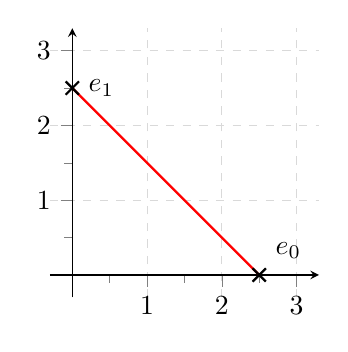
\begin{tikzpicture}
    \tikzstyle{point}=[thick,draw=black,cross out,inner sep=0pt,minimum width=4pt,minimum height=4pt]
    \begin{axis}[
        legend pos=south west,
        axis x line=middle,
        axis y line=middle,
        grid = major,
        width=5cm,
        height=5cm,
        grid style={dashed, gray!30},
        xmin=0,    % start the diagram at this x-coordinate
        xmax=3,    % end   the diagram at this x-coordinate
        ymin=0,    % start the diagram at this y-coordinate
        ymax=3,    % end   the diagram at this y-coordinate
        %xlabel=$x$,
        %ylabel=$y$,
        tick align=outside,
        minor tick num=-3,
        enlargelimits=true,
        tension=0.08]
      \addplot[domain=0:2.5, red, thick,samples=20] {-x+2.5};
      \node[point,label={[label distance=0cm]45:$e_0$}] at (axis cs:2.5,0) {};
      \node[point,label={[label distance=0cm]0:$e_1$}] at (axis cs:0,2.5) {};
    \end{axis}
\end{tikzpicture}
\end{document}
